\begin{figure}[htbp]
\section*{SON}
\centering
\begin{subfigure}[b]{0.95\textwidth}
\centering
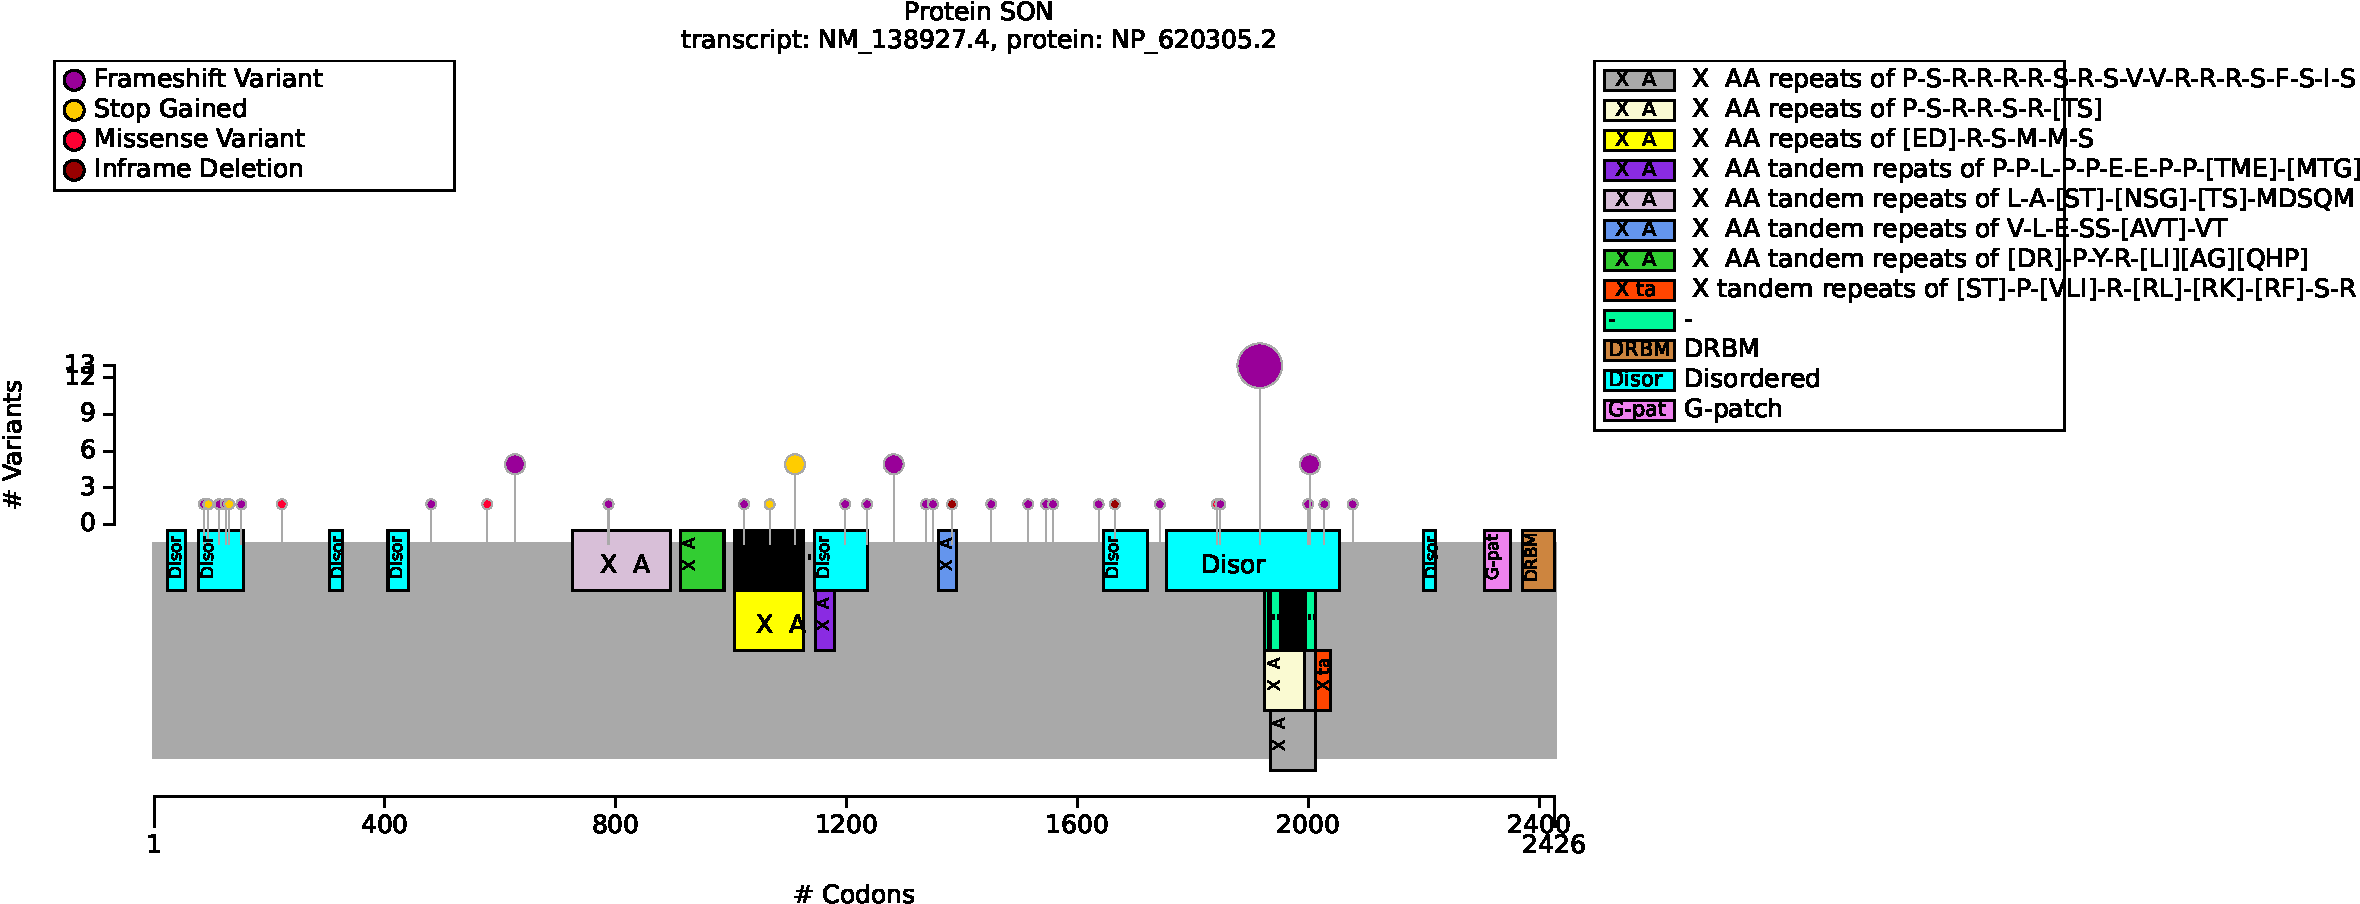
\includegraphics[width=\textwidth]{img/SON_protein_diagram.pdf} 
\captionsetup{justification=raggedright,singlelinecheck=false}
\caption{Distribution of variants in SON}
\end{subfigure}

\vspace{2em}

\begin{subfigure}[b]{0.95\textwidth}
\centering
\resizebox{\textwidth}{!}{
\begin{tabular}{llllrr}
\toprule
Genotype (A) & Genotype (B) & total tests performed & significant results\\
\midrule
missense & Other & 24 & 0\\
c.5753\_5756del & Other & 26 & 0\\
FEMALE & MALE & 27 & 0\\
\bottomrule
\end{tabular}
}
\captionsetup{justification=raggedright,singlelinecheck=false}
\caption{Fisher Exact Test performed to compare HPO annotation frequency with respect to genotypes.}
\end{subfigure}

\vspace{2em}

\caption{ The cohort comprised 52 individuals (26 females, 26 males). A total of 47 HPO terms were used to annotate the cohort. Disease diagnosis: ZTTK SYNDROME (OMIM:617140). Dingemans et al \cite{PMID_34521999} suggested a different pathomechanism for missense variants, but only our cohort only contains 3 individuals A total of 52 unique variant alleles were found in \textit{SON} (transcript: \texttt{NM\_138927.4}, protein id: \texttt{NP\_620305.2}).}
\end{figure}
